% Desarrollo

This chapter describes the process of design, implementation and configuration of the modular charging station and drone instrumentation. It details the methodologies and tools used to carry out the development, with a focus on creating an effective solution for the charging system.

\section{Design and Development of the Charging Station}
\subsection{Requirements}
The following outlines the technical specifications and requirements for the charging station, ensuring compatibility and efficiency for a drone swarm charging system:
    \begin{enumerate}
        \item The system must feature a modular and stackable design for integrating multiple charging stations.
        \item The system must take into account and adapt to the dimensions of the proposed drone for the application.
        \item The system must include an automatic mechanism for opening and closing to store the drone.
        \item The system must have a charging mechanism for the drone's battery.
        \item The system must incorporate a vision-based positioning method for the drone.
    \end{enumerate}

\subsection{Bill of Materials}
The following is the list of materials used for constructing the modular charging station. It is worth noting that the design and development of this project heavily relied on previously available resources and materials, enabling cost optimization and efficient use of existing supplies.
\begin{itemize}
    \item Aluminum Profiles
        \begin{itemize}
            \item \textbf{30 mm:}
            \begin{itemize}
            \item 4 x Profiles of 100 mm
            \item 4 x Profiles of 810 mm
            \item 6 x Profiles of 750 mm
            \end{itemize}
            \item \textbf{40 mm:}
            \begin{itemize}
            \item 2 x Profiles of 1040 mm
            \item 4 x Profiles of 560 mm
            \item 4 x Profiles of 830 mm
            \item 4 x Profiles of 1120 mm
            \end{itemize}
        \end{itemize}
    \item 16 x 3D-Printed Aluminum Profile Elbows
    \item Aluminum Profile Fasteners
    \item 2 x Telescopic Slide Rails
    \item 1 x 12V Motor
    \item 1 x 3D-Printed Motor Bracket
    \item 1 x V-Belt 1 m
    \item 2 x Type A Pulleys with 1/2" Inner Diameter
    \item 2 x Bearings with ID: 15 mm and OD: 35 mm
    \item 2 x 3D-Printed Bearing Housings
    \item 2 x 9 mm MDF Boards of 75x75 cm
    \item 8 x 3D-Printed MDF Spacers
    \item 1 x 12V Power Supply
    \item 1 x Arduino Mega
    \item 1 x Raspberry Pi 4
    \item 1 x BTS7960 H-Bridge
    \item 2 x Inductive Proximity Sensors
    \item 1 x Joystick
    \item 1 x WiFi Router
    \item 1 x BT3 Pro Compact Charger
    \item 1 x Cable Carrier 1 m
    \item 1 x Shaft
\end{itemize}

\subsection{CAD Design of the Charging Base}

To meet the modular/stackable design requirements and ensure compatibility with the drone's dimensions, the following CAD design was developed:

As shown in \ref{fig:cajon_interno}, the base known as the "internal drawer" was designed to serve as a platform for the drone's takeoff and landing. This design was created considering the drone's dimensions and ensuring the inclusion of adequate tolerances to prevent potential collisions. A 30 mm aluminum profile was used in this design, taking advantage of previously available materials. Additional profiles were also integrated horizontally in the middle of the drawer to support the rails.
        
        
Consequently, based on the dimensions of the previous blueprint, the "external drawer" was designed. This drawer serves to house the drone and the electronics of the charging station, as shown in \ref{fig:cajon_externo}.
    

Next, the dimensions of the drone's landing gear were considered to 3D print mechanical guides (\ref{fig:guias_mecanicas}) that help align the landing gear for proper magnetic connection with the charging system.
    

Using the designs from \ref{fig:cajon_interno} and \ref{fig:guias_mecanicas}, the complete design of the internal drawer was developed (\ref{fig:final_interno}). It includes two 9 mm MDF cuts measuring 810 mm x 810 mm and internal spacers with a height of 20 mm to protect the system's cables. 

        \begin{figure}[H]
            \centering
            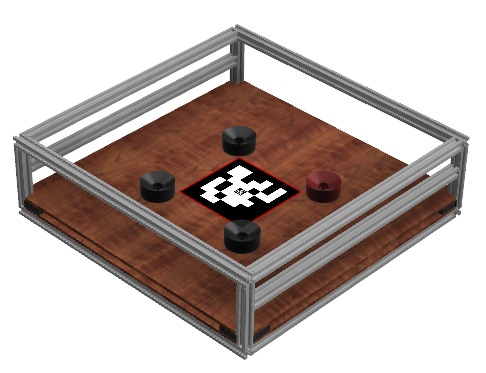
\includegraphics[width=0.6\textwidth]{pictures/CAJON_INTERNO_FINAL.jpeg}
            \caption{View of the internal drawer for the Charging Station.}
            \label{fig:final_interno}
        \end{figure}

The necessary CAD designs, as shown in \ref{fig:patas_estabilidad} and \ref{fig:inductive_holder}, were developed to ensure proper integration and adaptation of the various components of the charging station. These designs helped establish the essential dimensions, tolerances, and characteristics to ensure that each element fit precisely, guaranteeing that the charging station functioned efficiently and reliably.


Lastly, as part of the design process, a CAD model was developed to integrate the main components necessary for the proper functioning of the charging station. This final conceptual design, shown in \ref{fig:final_estacion}, represents the consolidation of initial ideas, the iterations performed, and the decisions made throughout the development. The model ensures the functionality, compatibility, and efficiency of the station, serving as a basis for manufacturing and implementing the system.

        \begin{figure}[H]
            \centering
            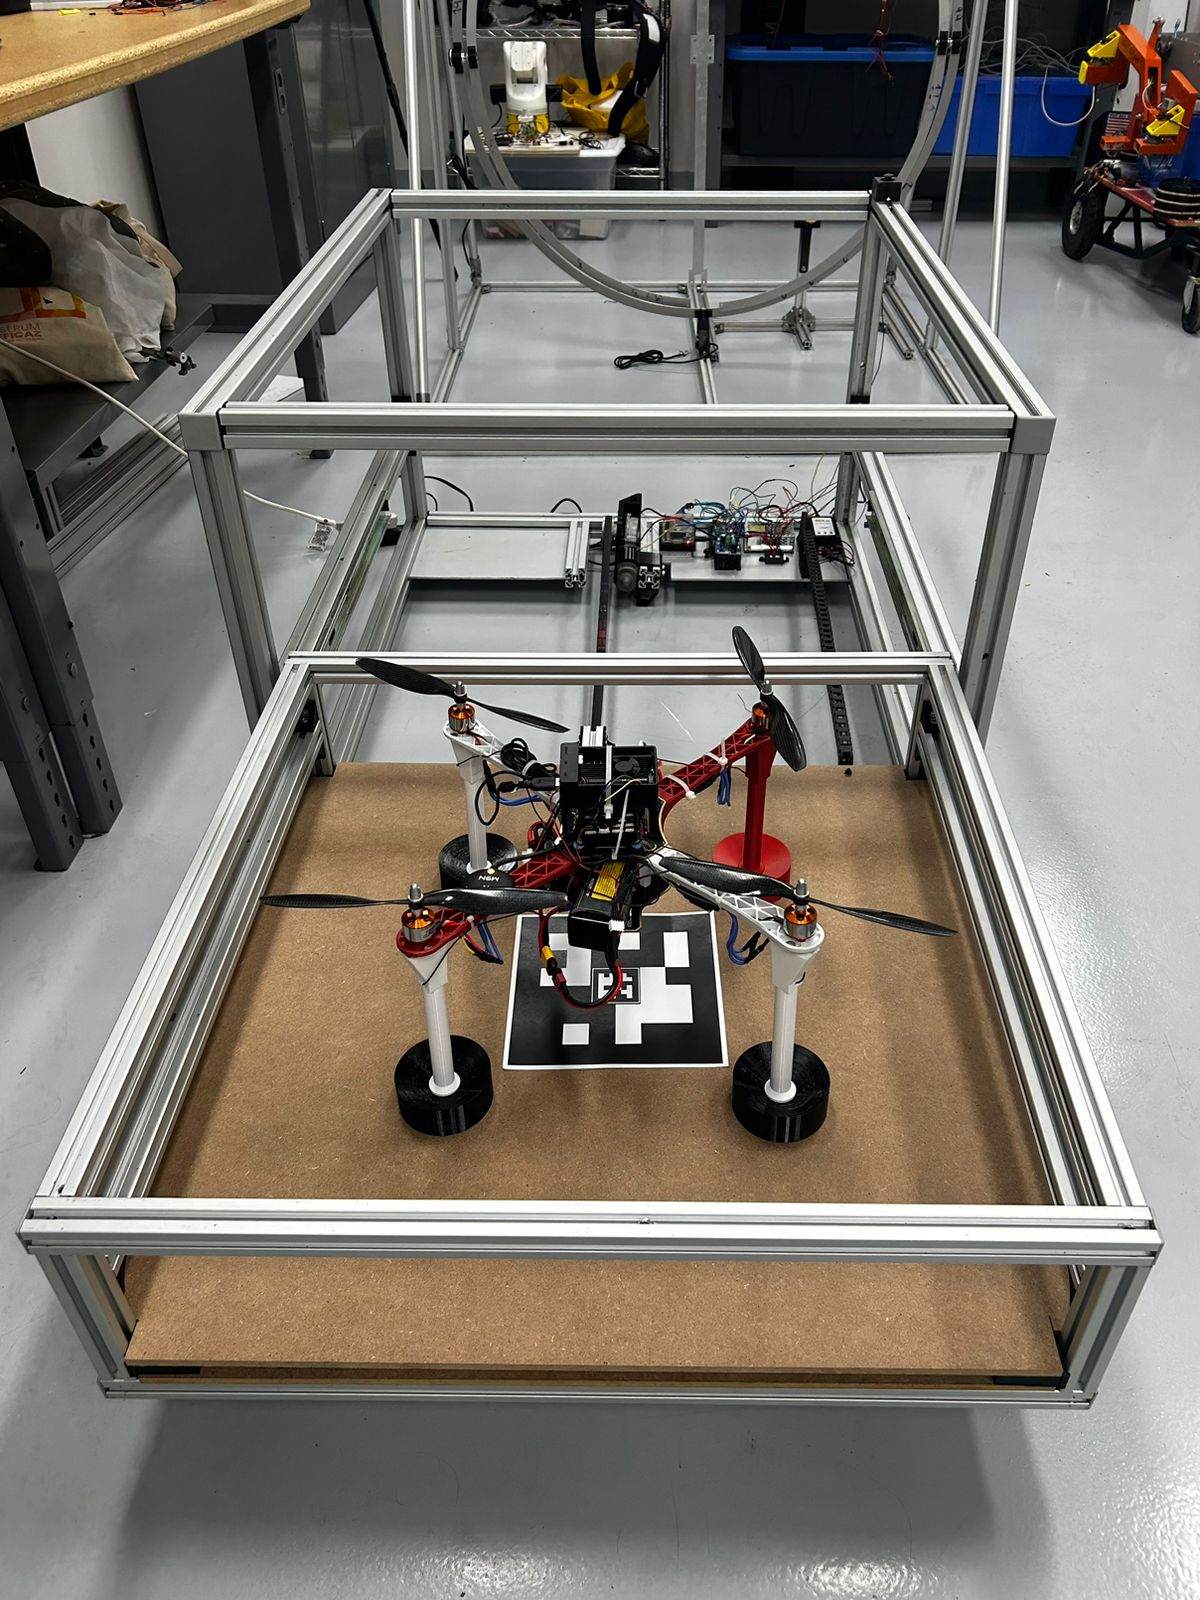
\includegraphics[width=0.5\textwidth]{pictures/ESTACION_FINAL.jpg}
            \caption{View of the Charging Station.}
            \label{fig:final_estacion}
        \end{figure}

\subsection{Selection and Implementation of the Drawer Movement Mechanism}

The design of the automatic drawer mechanism for the charging station went through several conceptual stages, considering different options to ensure efficient and cost-effective movement. Initially, a toothed belt mechanism, similar to those used in 3D printers, was proposed to allow precise forward and backward movement. However, this solution proved costly and complex due to the required dimensions. As an alternative, pistons were considered, but they further increased the project's costs. Finally, a V-belt and pulley system (Type A) was chosen due to its quick availability and significant cost reduction, achieving a balance between functionality, simplicity, and economy.

\subsubsection{Components and CAD Designs}
    \begin{enumerate}
        \item 12V Motor (see Appendix, Figure \ref{fig:motor}).
            
        \item Pulleys (see Appendix, Figure \ref{fig:polea_aluminio}).
    
        \item V-Belt Type A (see Appendix, Figure \ref{fig:banda_v}).
        
        \item Bearings (see Appendix, Figure \ref{fig:balero}).

        \item Bearing Housings (see Appendix, Figure \ref{fig:chumacera}).
        
        \item 12V Motor Mounts (see Appendix, Figures \ref{fig:soporte_motor} and \ref{fig:soporte_motor2}).
        
        \item V-Belt Holder for the internal drawer (see Appendix, Figures \ref{fig:suj_banda} and \ref{fig:suj_banda2}).
        
        \item Shaft (see Appendix, Figure \ref{fig:flecha}).
            
    \end{enumerate}

\subsubsection{V-Belt and Pulley Mechanism}

\begin{figure}[H]
    \centering
    \begin{minipage}{0.49\textwidth}
        \centering
        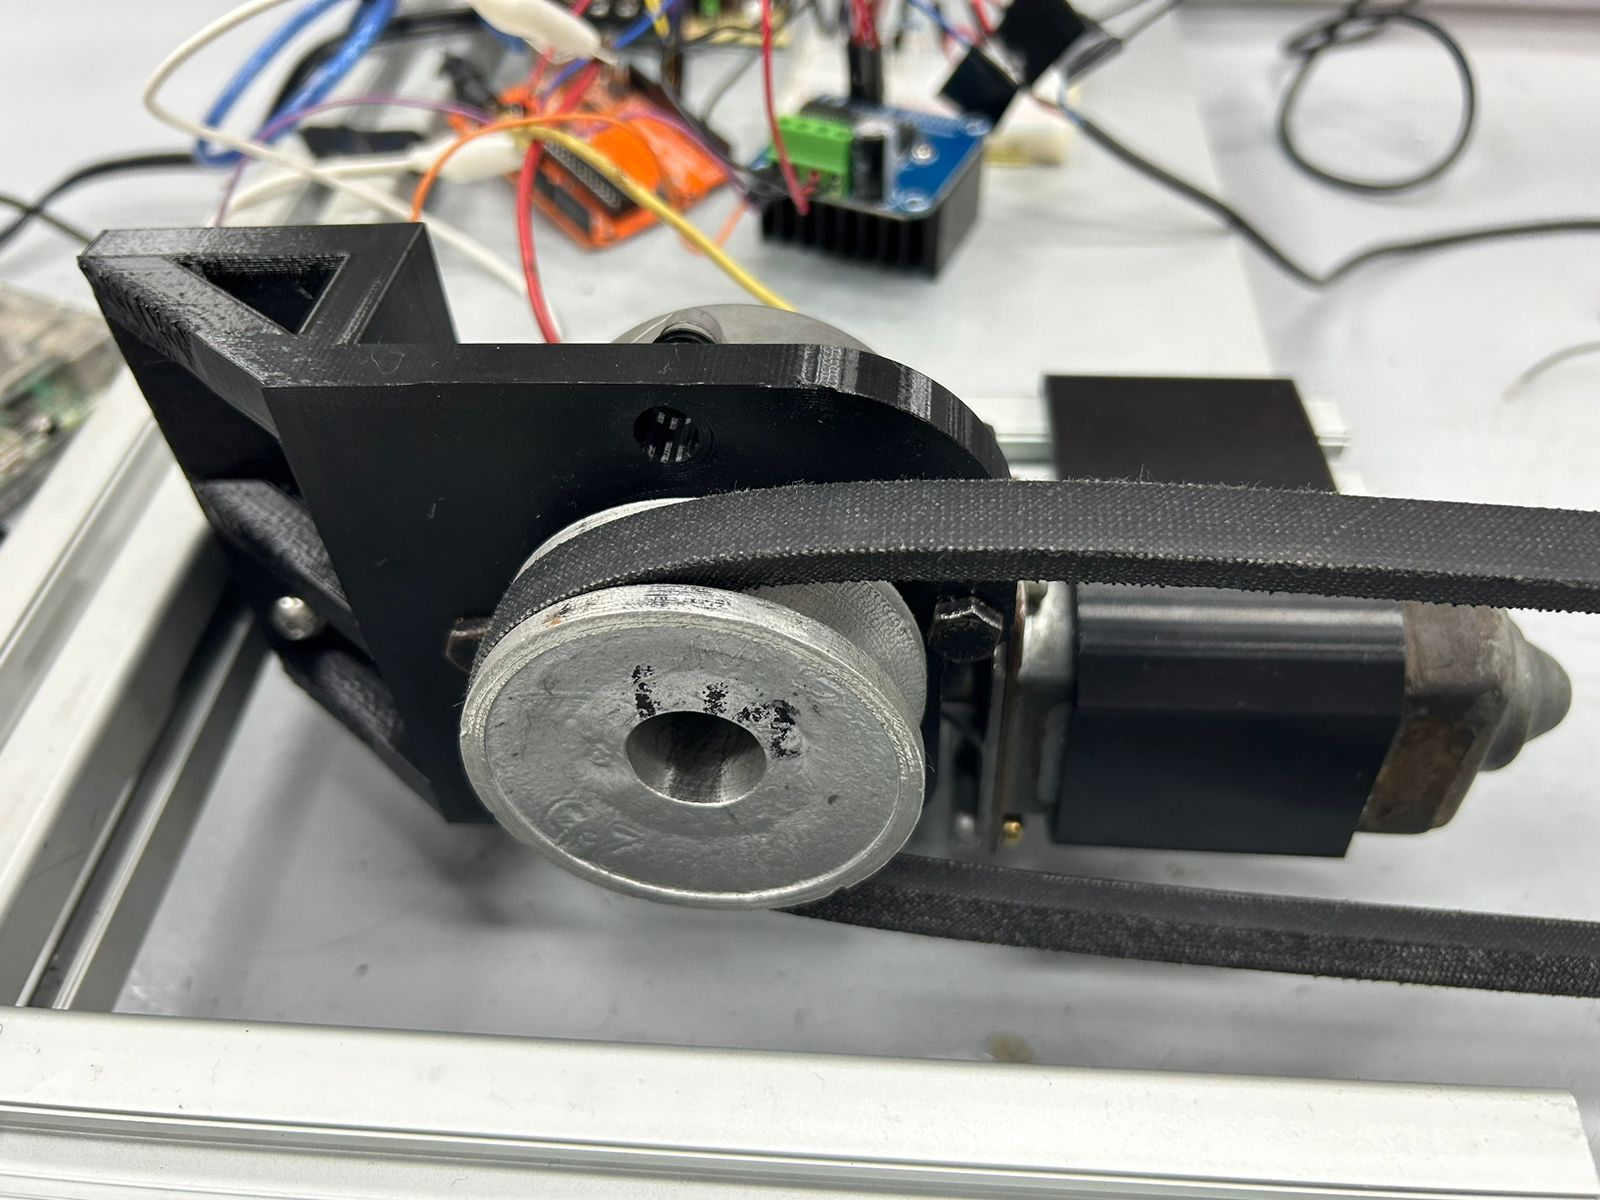
\includegraphics[width=\textwidth]{MECANISMO/MOTOR_MECANISMO.jpg}
        \caption{View of the internal drawer movement mechanism, showing the 3D-printed motor mounts and the motor with the pulley and belt integrated into the system.}
        \label{fig:motor_mecanismo}
    \end{minipage}%
    \hfill
    \begin{minipage}{0.49\textwidth}
        \centering
        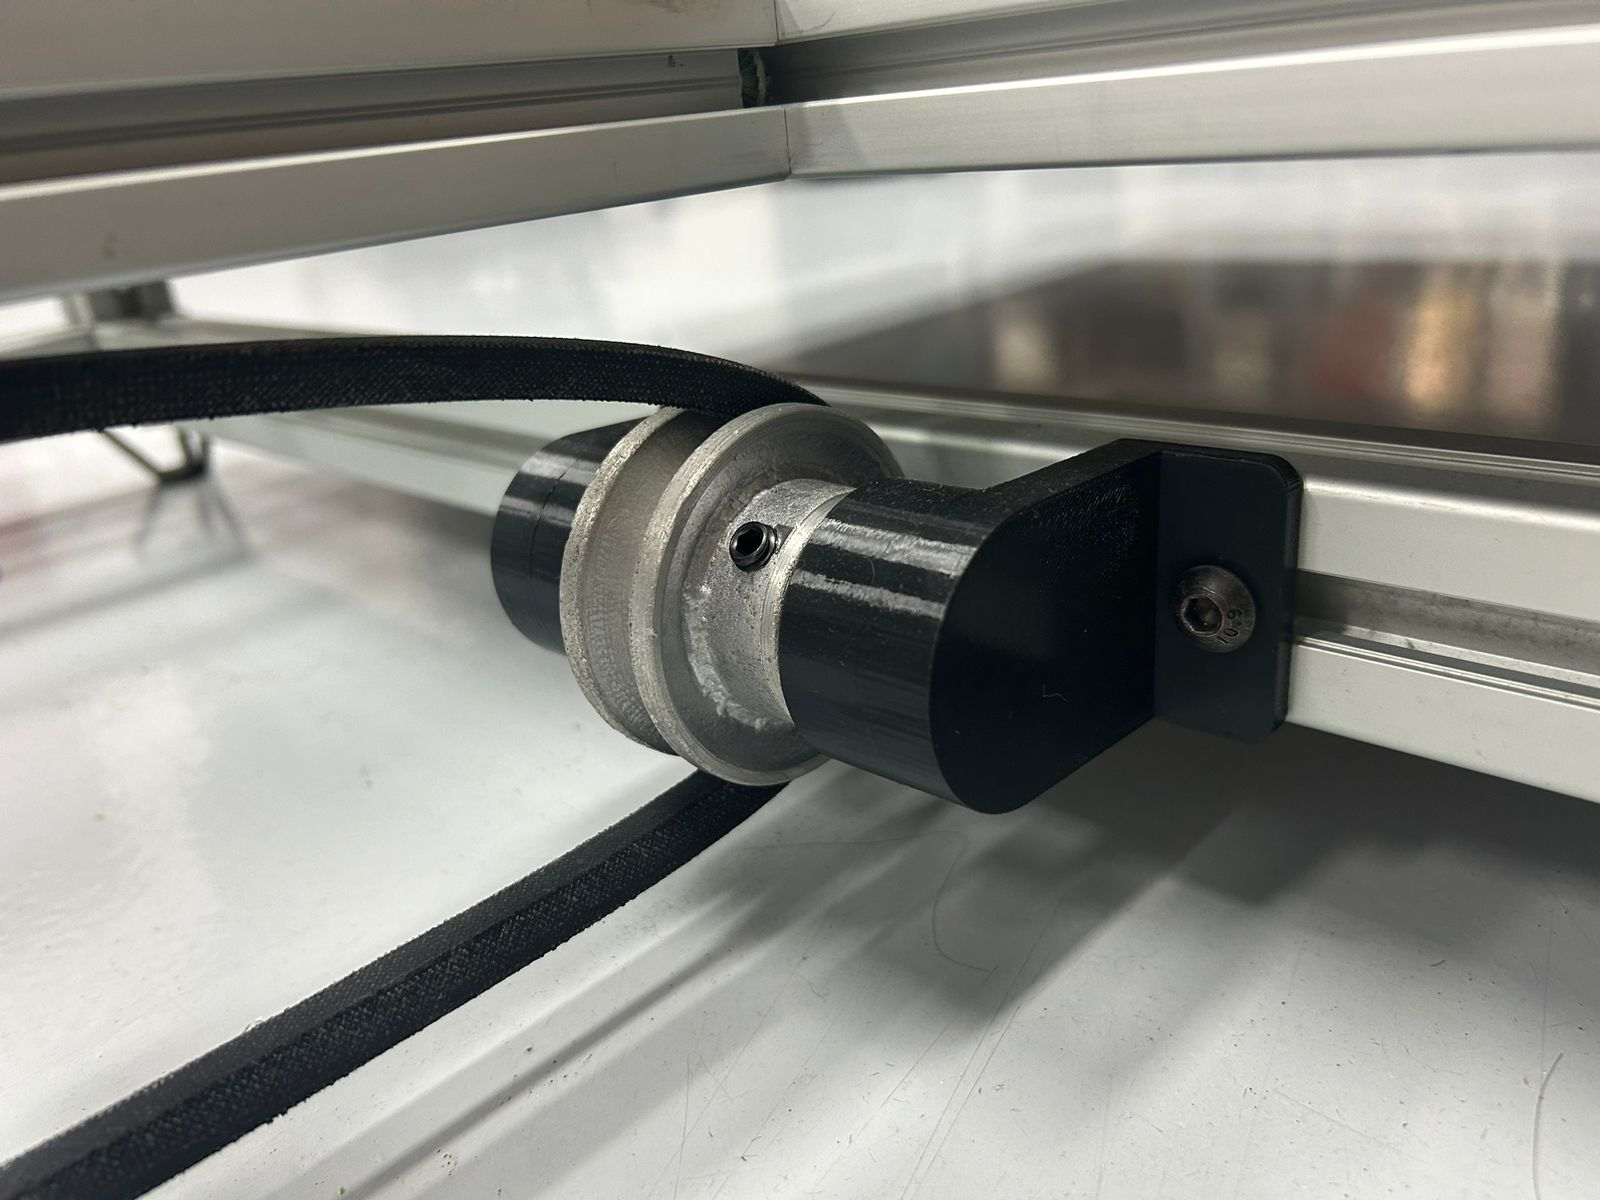
\includegraphics[width=\textwidth]{MECANISMO/MECANISMO_CHUMACERAS.jpg}
        \caption{View of the internal drawer movement mechanism, showing the 3D-printed bearing housings with...}
        \label{fig:mecanismo_chumaceras}
    \end{minipage}%
    \hfill
    \begin{minipage}{0.49\textwidth}
        \centering
        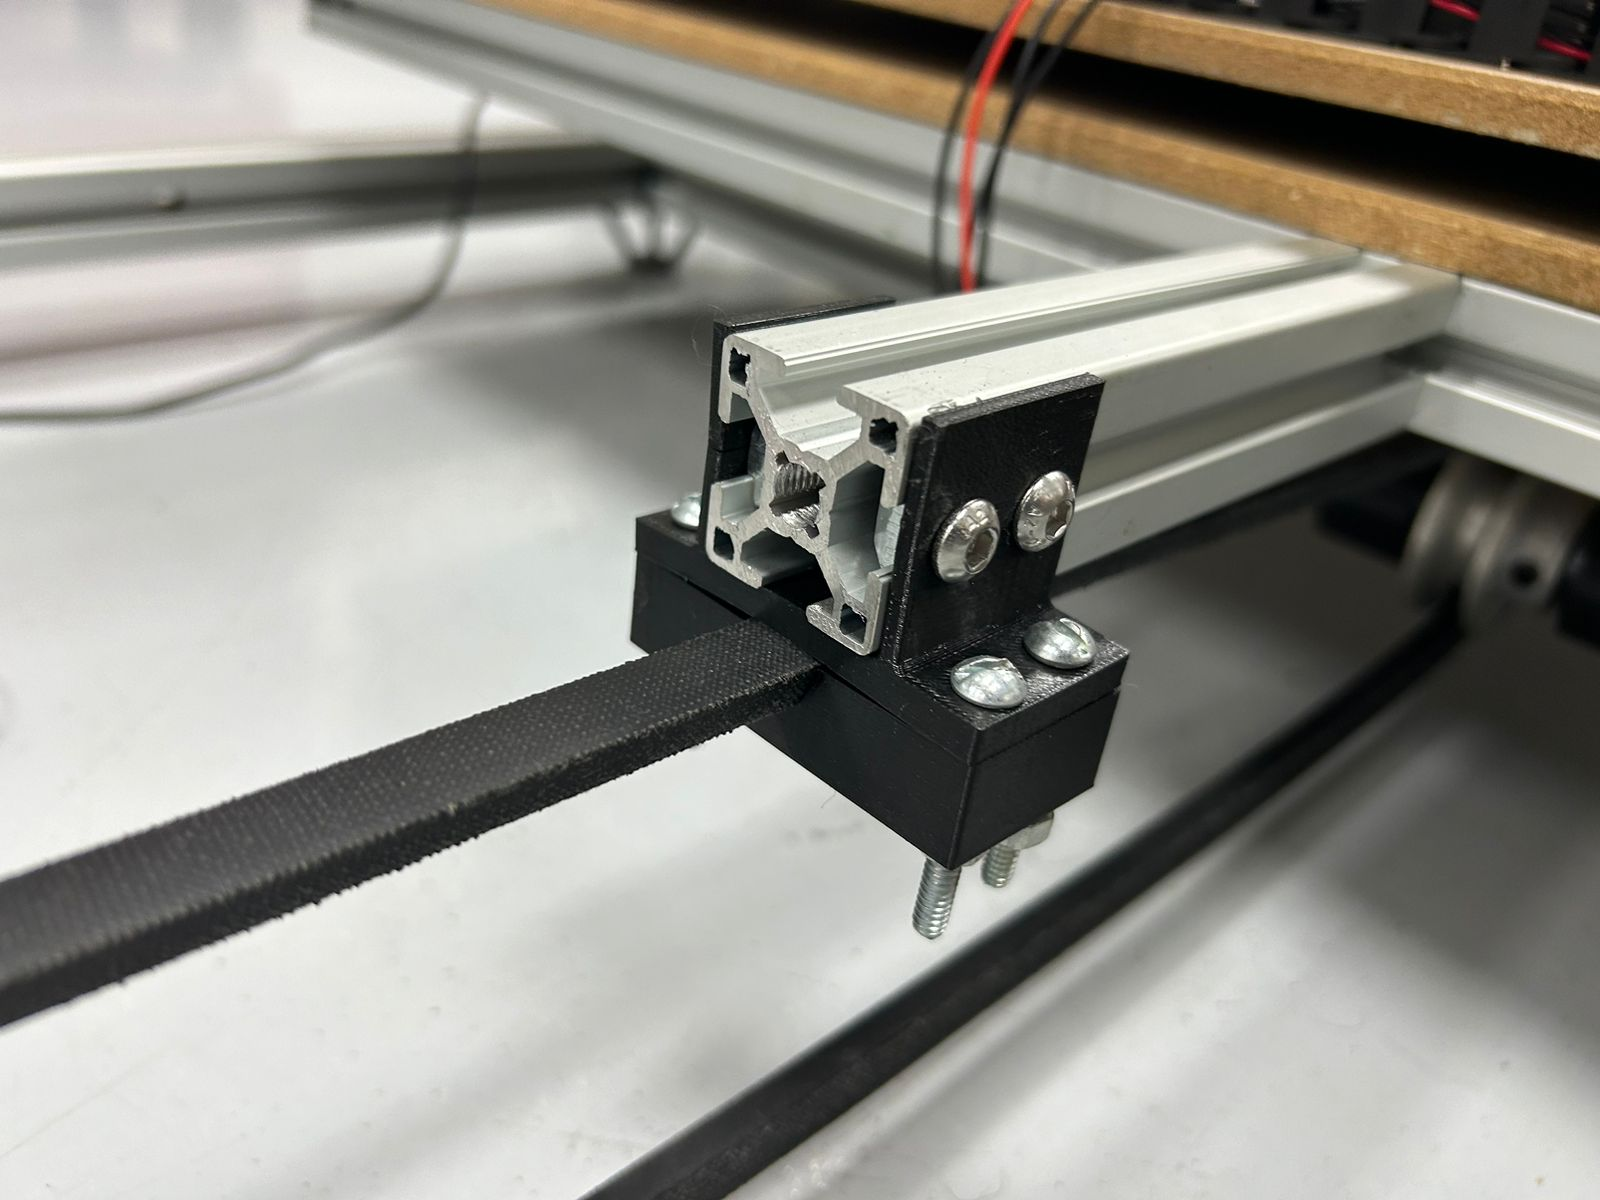
\includegraphics[width=\textwidth]{MECANISMO/MECANISMO_AGARRE.jpg}
        \caption{View of the internal drawer movement mechanism, showing the 3D-printed holder designed to secure the belt to the internal drawer.}
        \label{fig:mecanismo_agarre}
    \end{minipage}%
    \hfill
\end{figure}



\subsection{Manufacturing Process of the Charging Base Structure}

    \begin{enumerate}
        \item \textbf{Material Cutting:} To begin the manufacturing process, precise cuts were made on the aluminum profiles and MDF plates according to the dimensions specified in the bill of materials. This step is crucial to ensure that all pieces assemble correctly in the modular design. This process can be observed in Figure ? a).
            
        \item \textbf{Structure Assembly:} Once the pieces were cut, the main structure of the charging station was assembled using screws and nuts to secure the aluminum profiles and MDF plates with 3D-printed 20 mm spacers. It was verified that all components were aligned and leveled to ensure the stability and strength of the charging base. This is shown in Figures ? b) and c).
            
        \item \textbf{Installation of the Movement Mechanism:} After assembling the main structure, the V-belt and pulley mechanism was installed to enable the horizontal movement of the drawer. The pulleys, belt, and motor were placed in their predefined locations, ensuring that the movement system operated correctly and without obstructions. Figure ? d).
        
    \end{enumerate}


%%ANABI starts

\subsection{Electronic Circuit of the Charging Station}

    \subsubsection{Conection Diagram}
    
    \begin{figure}[H]
        \centering
        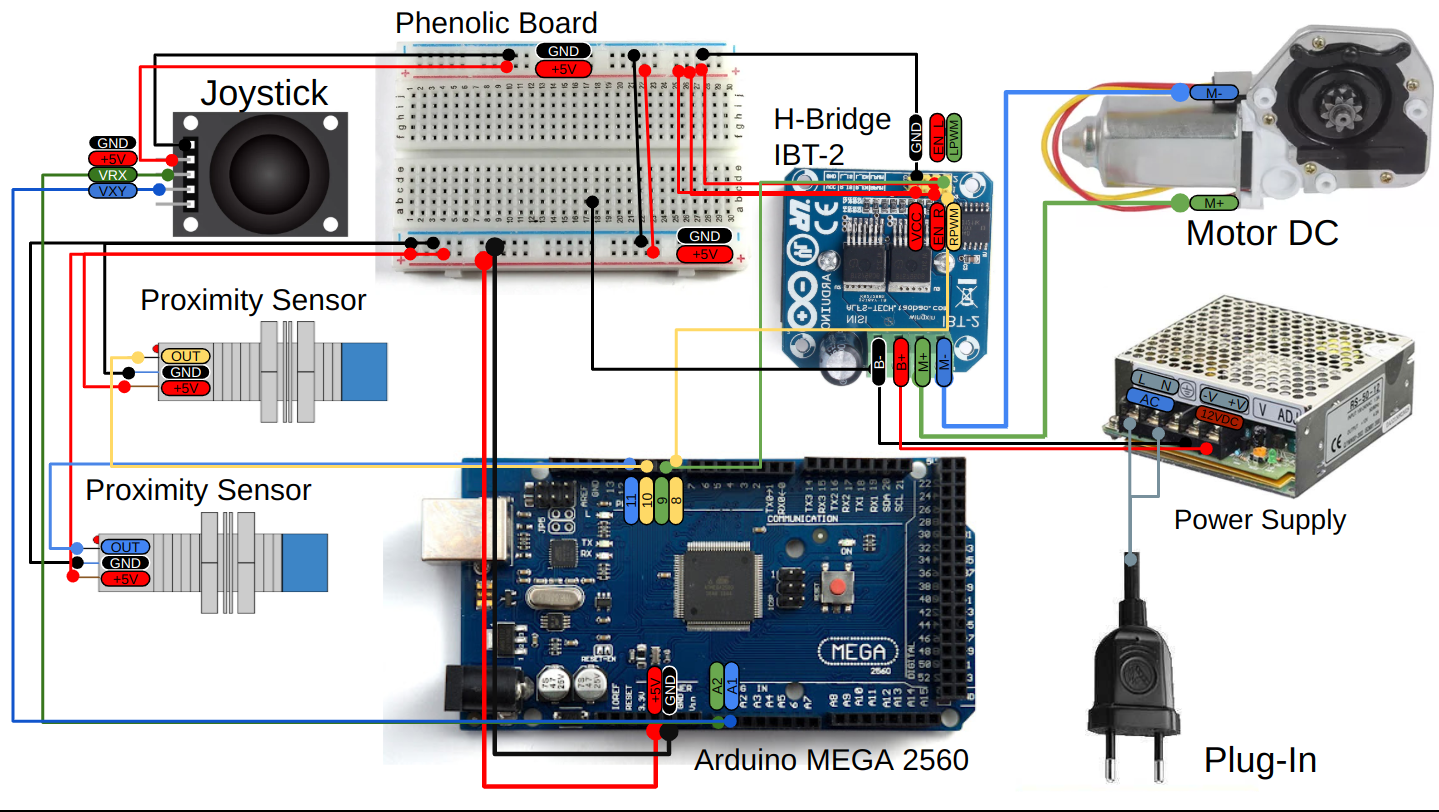
\includegraphics[width=0.7\textwidth]{pictures/station_electronics_diagram.png}
        \caption{Charging Station Electronics Diagram}
        \label{fig:station_electronics_diagram}
    \end{figure}
    
    \subsubsection{Circuit Construction}
    \begin{figure}[H]
        \centering
        %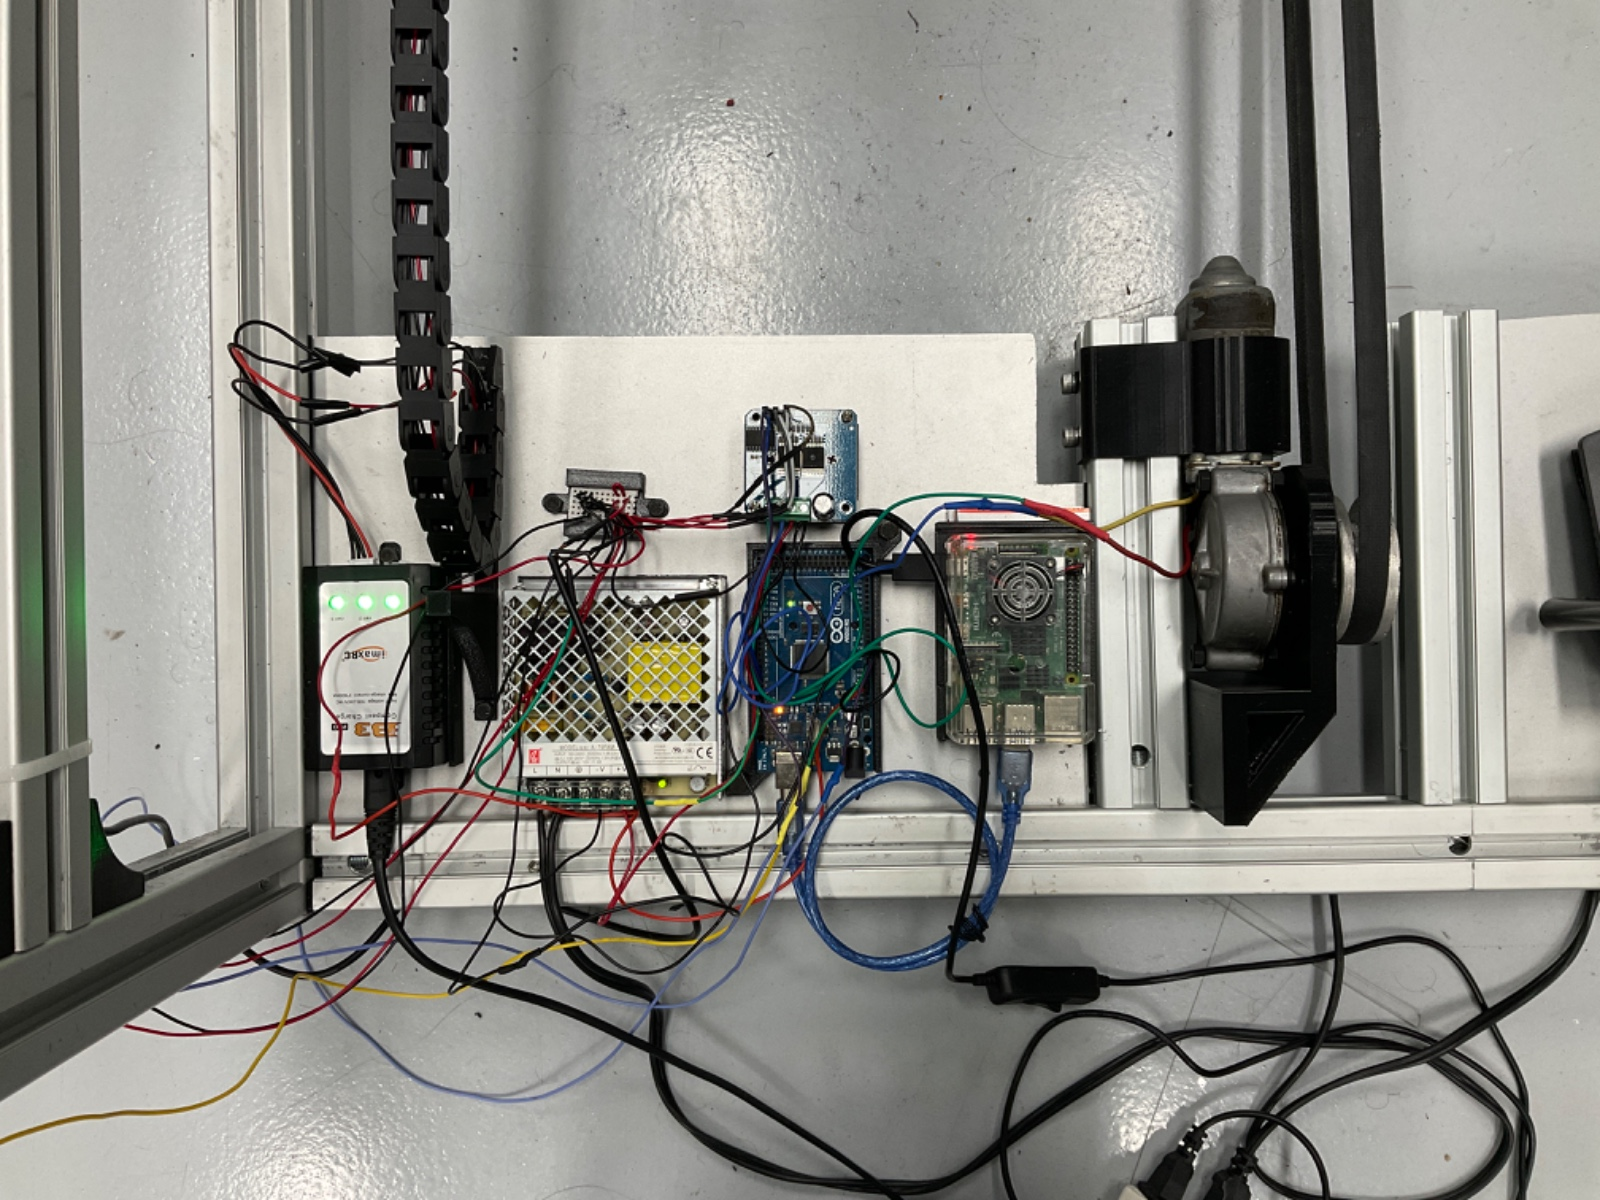
\includegraphics[width=0.5\textwidth]{pictures/station_electronics_circuit.png}
        \caption{Charging Station Electronics Circuit}
        \label{fig:station_electronics_circuit}
    \end{figure}
    
    \subsubsection{Circuit Programming}
    
    \paragraph{\textbf{General Description:}}
    
    
    The described circuit uses a joystick to control a motor that moves a drawer back and forth. The joystick is connected to a microcontroller (Arduino Mega 2560), which reads the joystick's Y-axis values to determine the direction in which the motor should move. Depending on the position of the joystick, the motor moves forward, backward or stops. In addition, limit switches are used to ensure that the motor stops when the drawer reaches its extreme positions.
    
    
    
    \paragraph{\textbf{Main Components}
    }
    \begin{itemize}
        \item \textbf{Arduino:} Microcontroller that manages the reading of the joystick values and controls the motor.
        \item \textbf{Joystick:} Analog input device that allows the user to control the direction of movement.
        \item \textbf{Motor and H-Bridge:} Driver system that moves the drawer. The H-bridge allows controlling the direction and speed of motion of the motor.
        \item \textbf{Limit Switches:} Sensors that detect when the drawer has reached its extreme positions (forward and reverse).
        \item \textbf{Power Supply:} Supplies power to the motor. The Arduino and RaspberryPi4 are supplied power by a plug-in charger.
    \end{itemize}
    
    
    \paragraph{\textbf{Arduino Code}
    }
    
    The Arduino code performs the following functions:
    
    \begin{enumerate}
        \item \textbf{Pin initialization:}
        \begin{itemize}
            \item The joystick pins (A1 for the Y-axis) are configured as inputs.
            \item Motor pins 9 and 8 are configured as outputs.
            \item The limit switch pins (10 and 11) are configured as inputs with internal pull-up resistors.
        \end{itemize}
        \item \textbf{Reading of Joystick:}
        \begin{itemize}
            \item At each loop cycle, the Arduino reads the analog value from the joystick's Y-axis.
            \item Depending on the value read, the Arduino decides whether the motor should move forward, backward or stop.
        \end{itemize}
        \item \textbf{Motor Control:}
        \begin{itemize}
            \item If the value of the joystick Y-axis is greater than 512 (middle position) and the forward limit switch is not pressed, the motor moves forward.
            \item If the Y-axis value is less than 512 and the backward limit switch is not pressed, the motor moves backward.
            \item If the Y-axis value is approximately 512 or any limit switch is pressed, the motor stops.
        \end{itemize}
        \item \textbf{Limit Switch Verification:}
        \begin{itemize}
            \item If the motor is moving forward and the forward limit detects  metal (the drawer), the motor stops.
            \item If the motor is moving backward and the backward limit switch detects  metal (the drawer), the motor stops.
    
        \end{itemize}
        
    \end{enumerate}
    
    %%%%%CODIGOOOOOOOO (??????)
    
    \paragraph{\textbf{Circuit Operation}
    }
    \begin{itemize}
        \item Initialization: At startup, the Arduino configures the pins and establishes serial communication for debugging.
    \item Continuous Readout: In the main loop, the Arduino continuously reads the value of the joystick Y-axis.
    \item Dynamic Control: Based on the value read, the Arduino controls the motor to move the drawer forward, backward or stop it.
    \item Safety Check: Limit switches ensure that the motor automatically stops when the drawer reaches its extreme positions, protecting the system from possible damage.
    \item Debugging: Joystick values and motor status are printed on the serial monitor for easy debugging and system tuning.
    \end{itemize}
    
    \paragraph{\textbf{Annex}
    }
    %\paragraph{
    The complete source code for both the Arduino and Raspberry Pi 4 is included in the appendices of this document, making it easy to review and modify as needed for implementation and control of the system.
    
    This approach ensures that the drawer moves in a precise and controlled manner based on the joystick position, providing an efficient solution for linear motion control using a motor and belt.

%%ANABI ENDS
    
\section{Drone Instrumentation}

\subsection{Specifications and Requirements}
To ensure compatibility and functionality within the charging system, the drone must meet the following specifications:
    \begin{itemize}
        \item The dimensions of the components must adapt to the frame of the open-architecture quadcopter purchased.
        \item The drone must have a charging circuit compatible with the charging station.
        \item The drone must include a camera and vision system for detecting Aruco markers.
        \item Localization sensors must be integrated for outdoor navigation.
        \item A microprocessor must be integrated as an auxiliary computer for data processing and communication with the charging station.
    \end{itemize}

\subsection{Bill of Materials for Drone Instrumentation}
    \begin{itemize} 
        \item 1 x Open-architecture quadcopter frame (F450)
        \item 1 x Flight controller (Pixhawk 6x) 
        \item 1 x Camera 
        \item 1 x Raspberry Pi 4 
        \item 1 x Voltage Regulator
        \item 4 x Brushless motors
        \item 4 x ESC Modules
        \item 1 x Lipo Battery 5200 mAh
        \item 1 x GPS module (compatible with the flight controller) 
        \item 1 x 3D Microprocessor Mount 
        \item 4 x 3D Drone Cover 1
        \item 4 x 3D Drone Cover 2
        \item 4 x 3D Drone landing gear
        \item 1 x 3D Camera Holder
    \end{itemize}


    \subsection{Drone CAD Designs} 
        The design and instrumentation of the drone began with the selection of an F450 open-source frame, a versatile and widely used option in drone development due to its compatibility with various components. The frame was equipped with brushless motors, ESC modules, a flight controller (Pixhawk 6x), a Raspberry Pi 4 as a companion computer, a GPS module, and a vision system. These components provided the drone with the necessary functionality for navigation, control, and interaction with the charging station.

        To adapt the drone for integration with the modular charging station, several 3D-printed components were designed and fabricated. These modifications improved the structural stability, protected critical elements, and ensured the drone could align with the station's charging system. Each component was custom-designed to fit the F450 frame and meet the specific requirements of the project.

        The following 3D-printed components were developed:

        \begin{itemize} 
            \item \textbf{1 x 3D Microprocessor Mount:}  
            A custom mount was created to securely hold the Raspberry Pi 5. This design ensures support and maintains accessibility for wiring and connectivity (see Appendix, Figure \ref{fig:rpi_mount}).
            
            \item \textbf{1 x 3D Camera Holder:}  
            This holder aligns the camera with the drone's forward direction, facilitating accurate detection of ArUco markers. The design includes adjustable angles to optimize the field of view (see Appendix, Figure \ref{fig:camera_holder}).

            \item \textbf{4 x 3D Drone Cover 1 and 4 x 3D Drone Cover 2:}  
            These two complementary covers were designed to secure the landing gear to the frame. **Drone Cover 1** and **Drone Cover 2** clasp the legs of the F450 frame from opposite sides, forming a secure connection. Together, they create a threaded joint, allowing the landing gear to be screwed into place. This modular approach ensures a firm attachment while enabling quick disassembly for maintenance or upgrades (see Appendix, Figures \ref{fig:drone_cover_1} and \ref{fig:drone_cover_2}).

            \item \textbf{4 x 3D Drone Landing Gear:}  
            The landing gear was designed to screw into the combined **Drone Cover 1** and **Drone Cover 2**, forming a robust and stable structure. The gear ensures improved balance during takeoff and landing, with anti-slip features and shock absorption to protect the frame and electronics on uneven surfaces (see Appendix, Figure \ref{fig:landing_gear}).
        \end{itemize}

        These 3D-printed designs allowed for significant improvements in the drone’s functionality and adaptability. Each component was tailored to ensure seamless integration with the charging station and to enhance the overall durability and performance of the drone. Detailed CAD designs and blueprints for these components can be found in the appendices of this document.

    
    \subsection{Power Distribution Circuit} 
        The power distribution circuit was designed to provide safe and stable power to the drone's critical components, including the motors, flight controller, Raspberry Pi, and camera. Below is a description of each section of the circuit:
    
        \begin{enumerate}
            \item \textbf{LiPo 3S Battery:} 
            A 3-cell lithium-polymer (LiPo) battery with a capacity of 5200 mAh, a nominal voltage of 11.1 V, and a discharge rate of 50C was selected. This battery is ideal for providing the necessary current to the motors and electronic components without compromising flight duration.
        
            \item \textbf{Power distribution to the motors:} 
            Power from the battery is distributed through a power distribution board that connects the battery to the four electronic speed controllers (ESC). Each ESC regulates the power sent to its respective A2212 10T motor, allowing precise control of the motor speeds.
        
            \item \textbf{XL4005 DC-DC Voltage Regulator:} 
            This regulator converts the battery’s 11.1 V output to 5 V, providing stable and safe power for the Raspberry Pi and the connected camera.
        
            \item \textbf{Pixhawk 6X RT Flight Controller:} 
            The flight controller is connected directly to the power distribution board to receive the necessary power. It also manages communication with the ESCs and other sensors on the drone, such as the GPS module (M9N) connected to the GPS1 port.
        
            \item \textbf{Raspberry Pi 5:} 
            The Raspberry Pi is powered through the voltage regulator and connects to the flight controller via a serial port to receive data and send commands to the system. It also manages the camera connected via USB, which captures images for real-time processing.
        
            \item \textbf{M9N GPS Module:} 
            This module connects to the Pixhawk controller via the GPS1 port to provide real-time positioning data outdoors, essential for drone navigation.
        
        \end{enumerate}
        
        \begin{center}
            \begin{figure}[H]
                \centering
                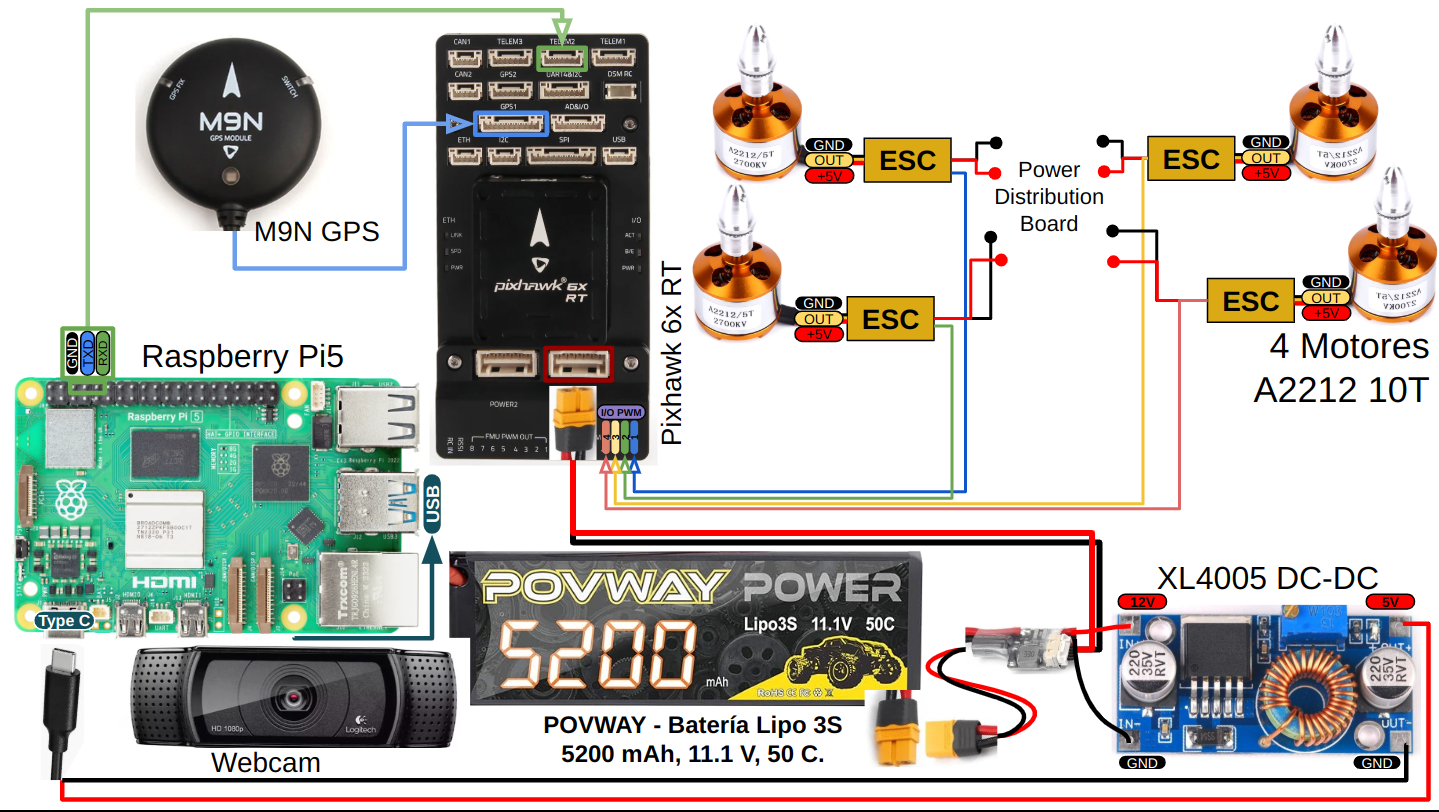
\includegraphics[width=0.8\textwidth]{pictures/drone_electronic_diagram.png}
                \caption{Diagram of the drone's power distribution circuit.}
            \end{figure}
        \end{center}
    
        

\section{Software Configuration}

\subsection{Configuration of the Ground Control Computer} 
The ground control computer was configured to monitor and process information from the drone's companion computer. Below are the steps performed for this configuration:

\begin{itemize}
    \item \textbf{Installation of ROS 2 Humble:} 
    Since the ground control computer uses Ubuntu 22.04, ROS 2 Humble was installed following the official instructions. The commands used were:
    \begin{verbatim}
    sudo apt update && sudo apt install -y software-properties-common
    sudo add-apt-repository universe
    sudo apt update
    sudo apt install -y ros-humble-desktop
    \end{verbatim}
    This included the installation of the necessary tools to develop and run applications in ROS 2 Humble.

    \item \textbf{Environment Setup:} 
    To simplify the use of ROS 2, the \texttt{~/.bashrc} file was configured. The following line was added to the end of the file:
    \begin{verbatim}
    source /opt/ros/humble/setup.bash
    \end{verbatim}
    Then, the following command was executed:
    \begin{verbatim}
    source ~/.bashrc
    \end{verbatim}

    \item \textbf{Cloning the GitHub Repository:} 
    A ROS 2 workspace was created, and the corresponding repository was cloned. The steps performed were:
    \begin{verbatim}
    mkdir -p ~/ros2_ws/src
    cd ~/ros2_ws/src
    git clone <repository_URL>
    cd ..
    colcon build
    \end{verbatim}

    \item \textbf{Configuration of \texttt{ROS\_DOMAIN\_ID}:} 
    To ensure proper communication between the ground control computer and the drone's companion computer, the \texttt{ROS\_DOMAIN\_ID} was set to 10. This was done by adding the following line to the \texttt{~/.bashrc} file:
    \begin{verbatim}
    export ROS_DOMAIN_ID=10
    \end{verbatim}
    Then, the following command was executed:
    \begin{verbatim}
    source ~/.bashrc
    \end{verbatim}
    
    \item \textbf{Verification of the ROS 2 Environment:} 
    Finally, the environment was verified to be properly configured using the following command:
    \begin{verbatim}
    ros2 doctor
    \end{verbatim}
    This confirmed that all necessary dependencies for ROS 2 Humble were installed and functioning correctly.
    
\end{itemize}

\subsection{Configuration of the Drone's Companion Computer} 
The Raspberry Pi 5 was configured as a companion computer for real-time data processing and communication with the charging station. The steps performed for its configuration are detailed below:

\begin{itemize}
    \item \textbf{Installation of Ubuntu 24.04:} 
    The Raspberry Pi Imager tool was used to install Ubuntu Server 24.04 LTS (64-Bit) on the SD card. During the initial setup, SSH was enabled, a user with a password was defined, and the Raspberry Pi was connected to the WiFi network.
    
    \item \textbf{Initial Connection and SSH:} 
    After inserting the SD card into the Raspberry Pi and connecting it to a monitor and keyboard, the device was powered on, and the configured credentials were entered. The IP address was obtained using the command:
    \begin{verbatim}
    hostname -I
    \end{verbatim}
    Using this information, an SSH connection was established from an external computer with:
    \begin{verbatim}
    ssh <user>@<IP>
    \end{verbatim}
    This allowed the Raspberry Pi to be configured remotely.
    
    \item \textbf{System Update:} 
    A full system update was performed using the following commands:
    \begin{verbatim}
    sudo apt update && sudo apt upgrade -y
    \end{verbatim}
    Additionally, \texttt{raspi-config} was installed to enable the serial port. This option was configured in \texttt{Interface Options > Serial Port} by selecting \texttt{No} and then \texttt{Yes}.
    
    \item \textbf{Modification of \texttt{bashrc} and ID Configuration:} 
    To ensure communication between all devices, the \texttt{ROS\_DOMAIN\_ID} was set to 10. The \texttt{~/.bashrc} file was edited with:
    \begin{verbatim}
    sudo vim ~/.bashrc
    \end{verbatim}
    At the end of the file, the following lines were added:
    \begin{verbatim}
    export ROS_DOMAIN_ID=10
    source /opt/ros/jazzy/setup.bash
    \end{verbatim}
    Changes were saved, and the following command was executed:
    \begin{verbatim}
    source ~/.bashrc
    \end{verbatim}
    
    \item \textbf{Installation of ROS 2 Jazzy:} 
    The official instructions were followed to install ROS 2 Jazzy on Ubuntu 24.04. The commands included:
    \begin{verbatim}
    sudo apt install -y software-properties-common
    sudo add-apt-repository universe
    sudo apt update
    sudo apt install -y ros-jazzy-desktop
    \end{verbatim}
    
    \item \textbf{Cloning the GitHub Repository:} 
    A ROS 2 workspace was created to integrate custom nodes. The steps performed were:
    \begin{verbatim}
    mkdir -p ~/ros2_ws/src
    cd ~/ros2_ws/src
    git clone <repository_URL>
    cd ..
    colcon build
    \end{verbatim}
    
    \item \textbf{Installation of MAVROS and MAVProxy:} 
    MAVROS and MAVProxy were installed for communication with the Pixhawk. The commands used were:
    \begin{verbatim}
    sudo apt install ros-jazzy-mavros ros-jazzy-mavros-extras
    sudo rosdep init
    rosdep update
    sudo apt install python3-mavproxy
    \end{verbatim}
    Additionally, geographic plugins were configured:
    \begin{verbatim}
    sudo apt install geographiclib-tools
    sudo geographiclib-get-geoids egm96-5
    \end{verbatim}
    
    \item \textbf{Communication Verification:} 
    To ensure MAVROS and MAVProxy worked correctly, MAVProxy was started first with:
    \begin{verbatim}
    mavproxy.py --master=/dev/ttyAMA0 --baudrate 921600
    \end{verbatim}
    Then, MAVROS was launched using:
    \begin{verbatim}
    ros2 launch mavros px4.launch fcu_url:=serial:///dev/ttyAMA0:921600
    \end{verbatim}
    Finally, the available topics were verified with:
    \begin{verbatim}
    ros2 topic list
    \end{verbatim}
    and communication was confirmed by observing the relevant topic messages.
    
    
\end{itemize}
    
\subsection{Configuration of the Ground Control Station} 
The configuration performed for the ground control station using QGroundControl and Mission Planner tools is detailed below. Both applications offer similar functionality, allowing for flight parameter visualization and management. However, since ArduPilot was used as the firmware, Mission Planner was prioritized due to its optimization for this system.
    
\begin{itemize}
    \item \textbf{Installation of Mission Planner and QGroundControl:} 
    Both tools were installed on the central computer for managing and monitoring the Pixhawk. Mission Planner was primarily used for its direct compatibility with ArduPilot, while QGroundControl was helpful for some initial configurations and redundant calibrations.
    
    \item \textbf{Sensor Calibration:} 
    Sensor calibration for the Pixhawk was performed using Mission Planner, following these steps:
    \begin{itemize}
        \item Access the calibration section in the \textit{Initial Setup} tab.
        \item Select the calibration option for each sensor:
        \begin{itemize}
            \item \textbf{Accelerometer:} The Pixhawk was placed in different orientations as instructed on-screen to ensure proper calibration.
            \item \textbf{Gyroscope:} The Pixhawk was kept stationary during the calibration process.
            \item \textbf{GPS:} Satellite reception was verified, and necessary parameters were adjusted for accurate positioning.
        \end{itemize}
    \end{itemize}
    \begin{figure}[H]
        \centering
        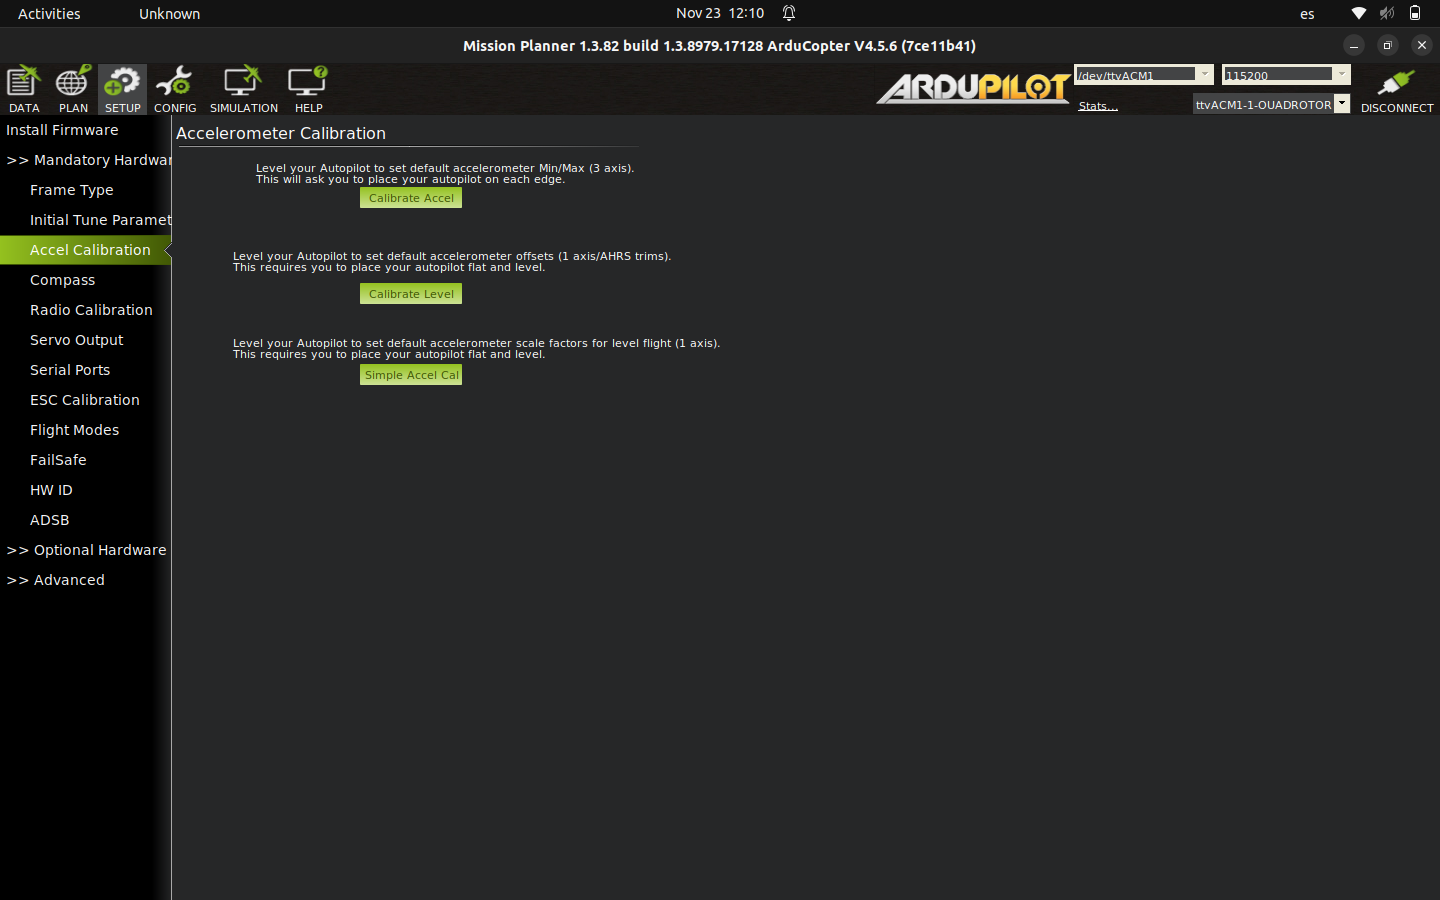
\includegraphics[width=0.8\textwidth]{pictures/mp_calibration.png}
        \caption{Image of sensor configuration in Mission Planner.}
    \end{figure}

    \item \textbf{Communication Parameters:} 
    To establish communication between the Raspberry Pi and the Pixhawk via MAVROS and MAVLink, the following parameter adjustments were made using Mission Planner:
    \begin{itemize}
        \item \texttt{SERIAL2\_PROTOCOL}: Set to 2 to enable MAVLink.
        \item \texttt{SERIAL2\_BAUD}: Set to 921600 to match the Raspberry Pi configuration.
        \item \texttt{SYS\_ID}: Set to the corresponding ID to ensure proper system communication.
    \end{itemize}
\end{itemize}

\section{Vision System}
\subsection{Specifications and Requirements} 
The vision system must meet the following requirements to ensure accurate detection of Aruco markers:
    \begin{itemize}
        \item Obtain the intrinsic and extrinsic calibration matrices of the camera.
        \item Generate and detect Aruco markers of various sizes in real time.
    \end{itemize}

\subsection{Camera Calibration} 
The camera calibration process was carried out using a Python script with the OpenCV library. This procedure is detailed below, combining code snippets and the images obtained at each stage. The full code can be found in the appendices of the document.

    \begin{enumerate}
        \item \textbf{Image Capture:} 
        Multiple images of the chessboard were collected from different angles and distances to cover the entire field of view of the camera. These images exhibited inherent lens distortions, as shown in Figure \ref{fig:imagen_descalibrada}.

        \begin{center}
            \begin{figure}[H]
                \centering
                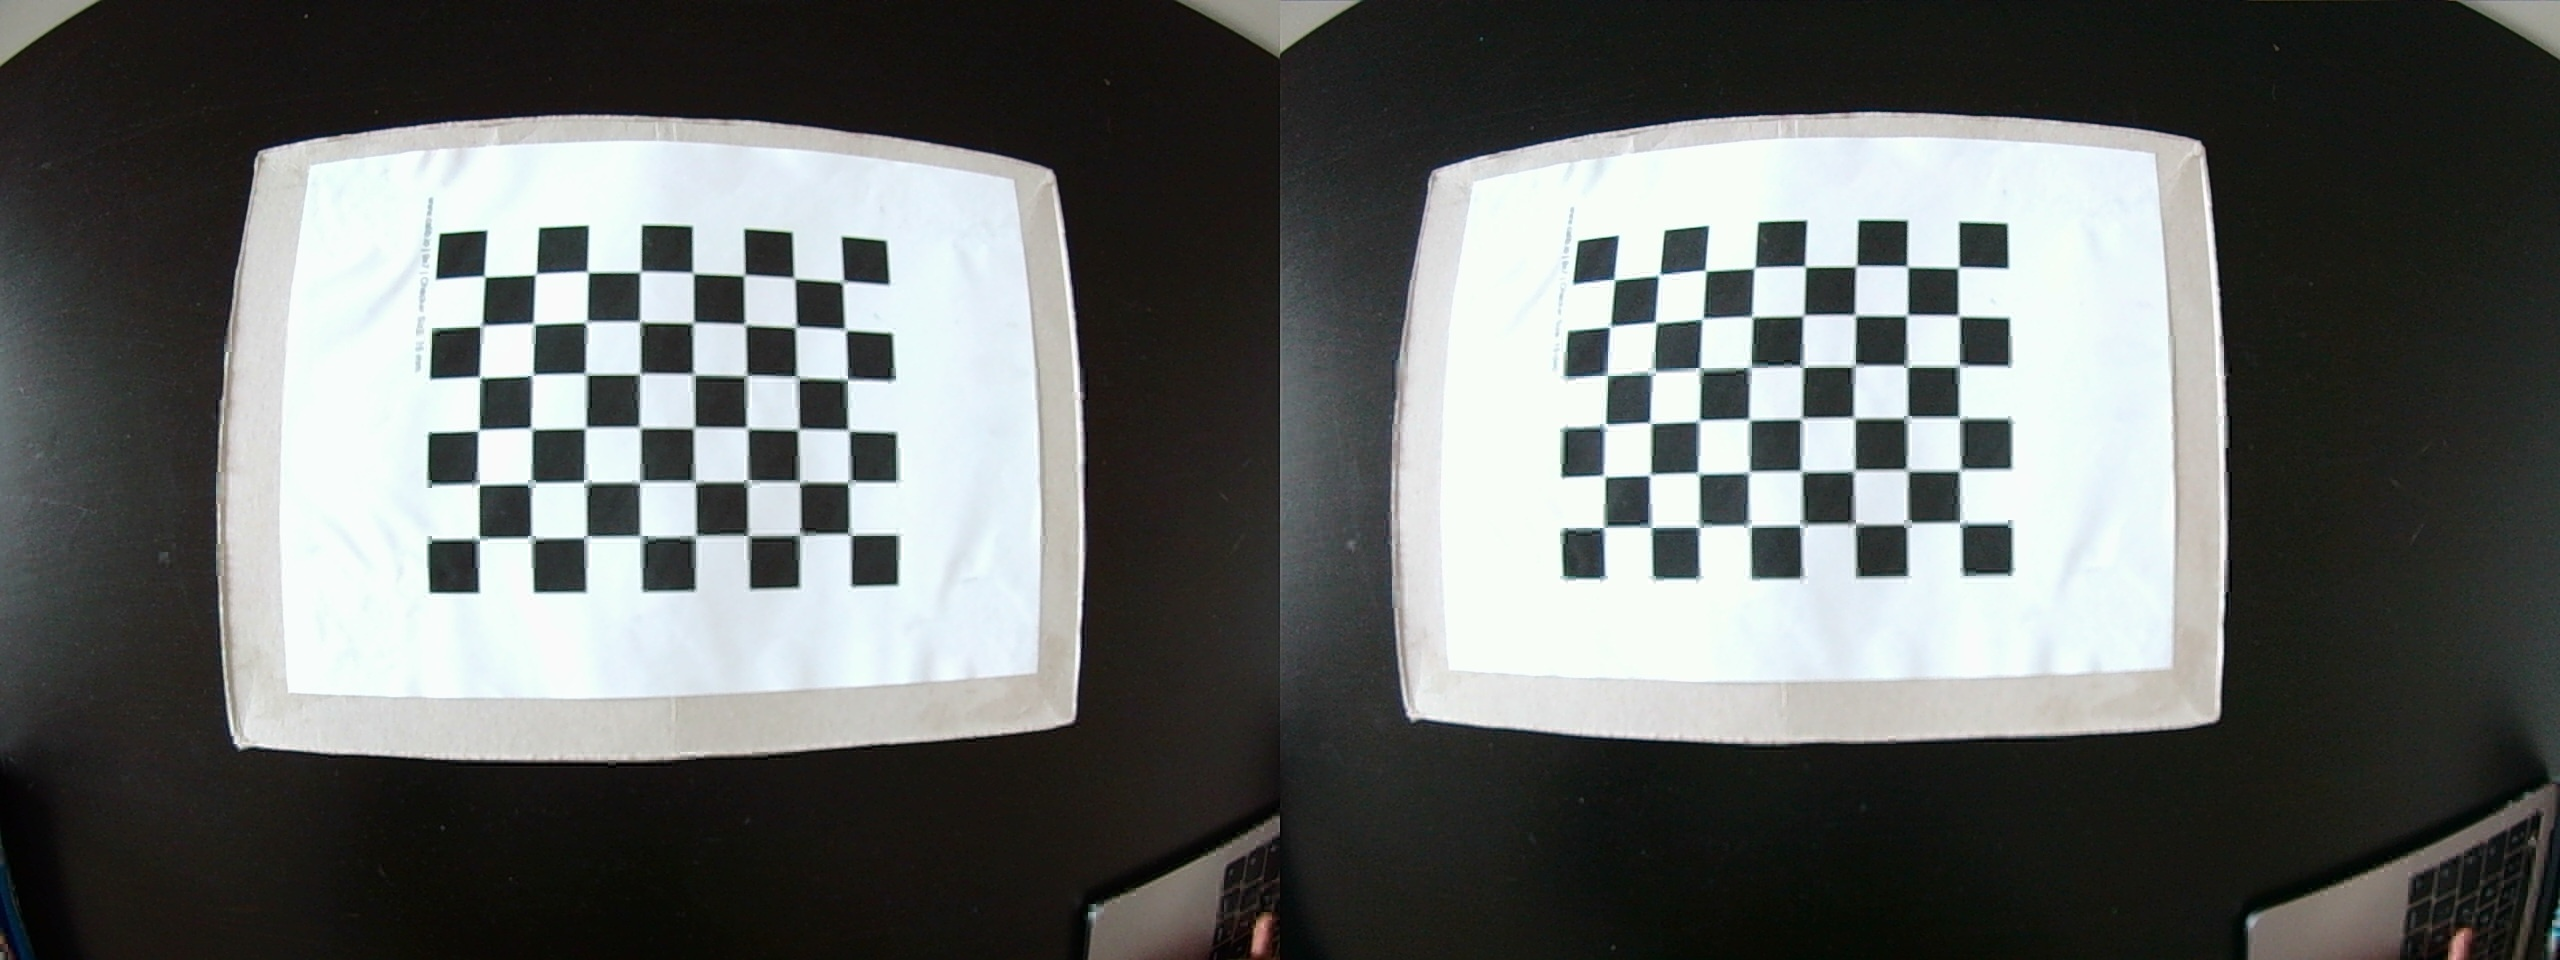
\includegraphics[width=0.8\textwidth]{pictures/imagen_descalibrada.jpg}
                \caption{Example of an uncalibrated image captured during the process.}
                \label{fig:imagen_descalibrada}
            \end{figure}
        \end{center}
    
        \item \textbf{Corner Detection:} 
        The script detected the internal corners of the chessboard using the \texttt{cv2.findChessboardCorners} function. The detected corners were then refined with \texttt{cv2.cornerSubPix}, and the calibration images were overlaid with the detected lines, as shown in Figure \ref{fig:det_ejemplos}.
        \begin{verbatim}
        ret, corners = cv2.findChessboardCorners(gray, (ncols, nrows), None)
        corners2 = cv2.cornerSubPix(gray, corners, (11, 11), (-1, -1), criteria)
        \end{verbatim}
        \begin{center}
            \begin{figure}[H]
                \centering
                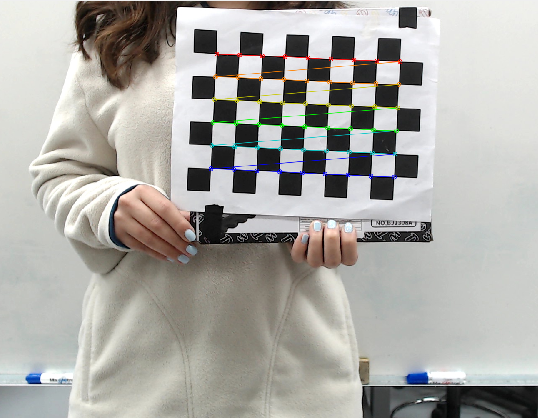
\includegraphics[width=0.8\textwidth]{pictures/calib_predictions.png}
                \caption{Detection and refinement of chessboard corners.}
                \label{fig:det_ejemplos}
            \end{figure}
        \end{center}
    
        \item \textbf{Camera Calibration:} 
        Using \texttt{cv2.calibrateCamera}, the camera's intrinsic parameters and distortion coefficients were calculated. These parameters allow for the correction of distortions in the captured images. Figure \ref{fig:imagen_calibrada} shows the result after applying these parameters.
        \begin{verbatim}
        ret, mtx, dist, rvecs, tvecs = cv2.calibrateCamera(objpoints, 
                                                           imgpoints, 
                                                           img_size, 
                                                           None, 
                                                           None)
        \end{verbatim}
        Where:
        \begin{itemize}
            \item \texttt{mtx}: Camera intrinsic matrix.
            \item \texttt{dist}: Distortion coefficients.
            \item \texttt{rvecs}, \texttt{tvecs}: Rotations and translations.
        \end{itemize}
        \begin{center}
            \begin{figure}[H]
                \centering
                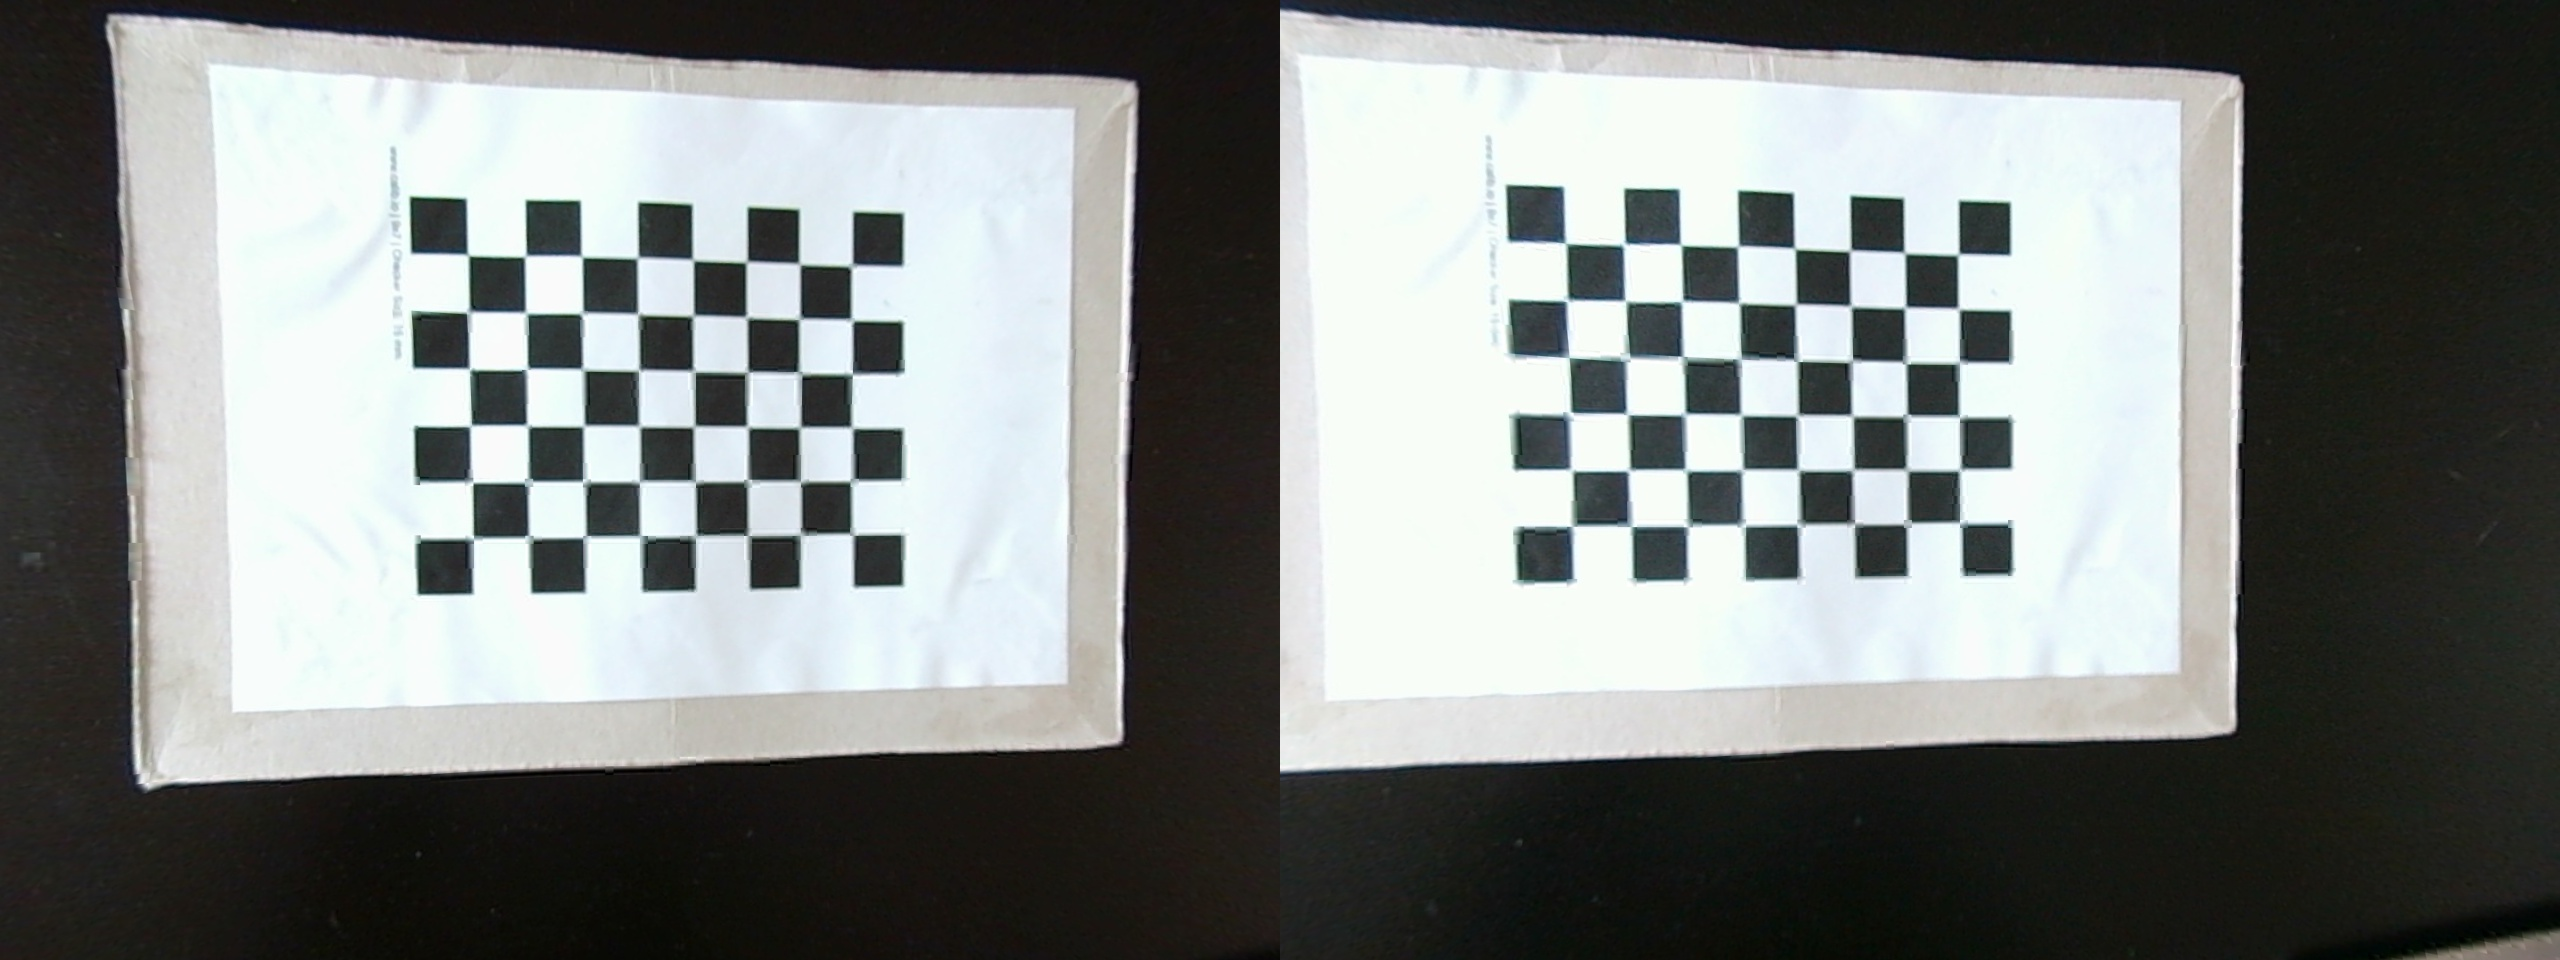
\includegraphics[width=0.8\textwidth]{pictures/imagenes_calibradas.jpg}
                \caption{Calibrated image after applying the obtained parameters.}
                \label{fig:imagen_calibrada}
            \end{figure}
        \end{center}
    
        \item \textbf{Calibration Error Calculation:} 
        The accuracy of the model was verified by calculating the average error using \texttt{cv2.projectPoints}. This calculation compares the detected and projected corners.
        \begin{verbatim}
        error = cv2.norm(imgpoints[i], imgpoints2, cv2.NORM_L2) / len(imgpoints2)
        print("Total error: {}".format(mean_error / len(objpoints)))
        \end{verbatim}
    
        \item \textbf{Parameter Storage:} 
        The obtained calibration parameters were saved in a JSON file for reuse in future image correction processes.
        \begin{verbatim}
        data = {"camera_matrix": mtx.tolist(), 
                "distortion_coefficients": dist.tolist()}
        with open(output_path, "w") as file:
            json.dump(data, file, indent=4)
        \end{verbatim}
    \end{enumerate}


\subsection{Generation of ArUco Markers} 
Custom ArUco markers were generated for the system, including specific sizes and patterns. In particular, embedded markers were created, where an inner marker is embedded within an outer marker to maximize detection accuracy. The step-by-step process is described below, highlighting important parts of the code used. The full code can be found in the appendices of the document.

    \begin{enumerate}
        \item \textbf{Loading the ArUco Dictionary:} 
        The predefined \texttt{DICT\_6X6\_250} dictionary from OpenCV was used, suitable for generating markers with different patterns and levels of detail.
        \begin{verbatim}
        aruco_dict = aruco.getPredefinedDictionary(aruco.DICT_6X6_250)
        \end{verbatim}
    
        \item \textbf{Generation of the Outer Marker:} 
        A size of 220 pixels (\texttt{outer\_marker\_size}) was defined for the outer marker, and it was generated with a specific ID (\texttt{outer\_marker\_id}). This allowed for creating a large marker to serve as a container.
        \begin{verbatim}
        outer_marker = aruco.generateImageMarker(aruco_dict, 
                                                    outer_marker_id, 
                                                    outer_marker_size)
        \end{verbatim}
        \begin{center}
            \begin{figure}[H]
                \centering
                
\includegraphics[width=0.4\textwidth]{pictures/aruco_marker_5.png}
                \caption{Generated outer ArUco marker.}
            \end{figure}
        \end{center}
    
        \item \textbf{Generation of the Inner Marker:} 
        The inner marker was generated with a size of 50 pixels (\texttt{inner\_marker\_size}) and a specific ID (\texttt{inner\_marker\_id}). This marker was designed to be embedded within the outer marker.
        \begin{verbatim}
        inner_marker = aruco.generateImageMarker(aruco_dict, 
                                                    inner_marker_id, 
                                                    inner_marker_size)
        \end{verbatim}

        \begin{center}
            \begin{figure}[H]
                \centering
                
\includegraphics[width=0.2\textwidth]{pictures/aruco_marker_100.png}
                \caption{Inner marker with added white border.}
            \end{figure}
        \end{center}
    
        \item \textbf{Adding a White Border Around the Inner Marker:} 
        A one-pixel white border was added around the inner marker using \texttt{cv2.copyMakeBorder}, which facilitates embedding and improves visibility under varying lighting conditions.
        \begin{verbatim}
        inner_marker_with_border = cv2.copyMakeBorder(
            inner_marker,
            top=border_size,
            bottom=border_size,
            left=border_size,
            right=border_size,
            borderType=cv2.BORDER_CONSTANT,
            value=255  # White
        )
        \end{verbatim}
        
    
        \item \textbf{Embedding the Inner Marker into the Outer Marker:} 
        The central position was calculated to embed the bordered inner marker into the outer marker. The outer marker was modified to include a black background in the center before inserting the bordered inner marker.
        \begin{verbatim}
        center_position = (outer_marker_size - inner_marker_with_border_size) // 2
        e_aruco_marker[center_position:center_position + inner_marker_with_border_size,
                        center_position:center_position + inner_marker_with_border_size] = 0
        e_aruco_marker[center_position:center_position + inner_marker_with_border_size,
                        center_position:center_position + inner_marker_with_border_size] = inner_marker_with_border
        \end{verbatim}
        \begin{center}
            \begin{figure}[H]
                \centering
                
\includegraphics[width=0.4\textwidth]{pictures/embedded_aruco.png}
                \caption{Generated embedded ArUco marker.}
            \end{figure}
        \end{center}
    
        \item \textbf{Saving the Embedded Marker:} 
        Finally, the generated marker was saved as a PNG image for later use.
        \begin{verbatim}
        cv2.imwrite(f'embedded_aruco_marker_{outer_marker_id}_{inner_marker_id}.png', 
                    e_aruco_marker)
        \end{verbatim}
    \end{enumerate}    

\subsection{Real-Time Detection of e-ArUco Markers} 
The system was designed to detect ArUco markers in real-time using images captured by a camera attached to the drone. This process was carried out via a ROS 2 node that processes images and estimates the pose of the markers relative to the camera. The full code is included in the appendices of the document. Below is the step-by-step description of the system:

    \begin{enumerate}
        \item \textbf{Image Publishing from the Drone:} 
        The companion computer on the drone publishes compressed images captured by the camera to a ROS 2 topic (\texttt{/camera\_image/compressed}). These images are sent to the ground computer for processing.
    
        \item \textbf{Image Reception on the Ground Computer:} 
        A node on the ground computer subscribes to the images published by the drone and performs the following tasks:
        \begin{itemize}
            \item Converts the compressed images into matrices for processing with OpenCV.
            \item Resizes the images and converts them to grayscale to optimize detection.
        \end{itemize}
    
        \item \textbf{Aruco Marker Detection:} 
        The OpenCV library is used to detect the ArUco markers present in the image. The steps include:
        \begin{itemize}
            \item Using the \texttt{DICT\_6X6\_250} dictionary to identify specific markers.
            \item Calculating the corners of the detected markers using \texttt{aruco.detectMarkers}.
            \item Drawing the detected markers for visualization.
        \end{itemize}
        \begin{center}
            \begin{figure}[H]
                \centering
                %\includegraphics[width=0.8\textwidth]{pictures/detection_arucos.png}
                %\caption{Detection of ArUco markers in the processed image.}
            \end{figure}
        \end{center}
    
        \item \textbf{Pose Estimation:} 
        For each detected marker, its position and orientation in space relative to the camera were calculated using the \texttt{aruco.estimatePoseSingleMarkers} function, which returns:
        \begin{itemize}
            \item \texttt{tvec}: Translation vector (\textit{x}, \textit{y}, \textit{z}) in meters.
            \item \texttt{rvec}: Rotation vector, converted to Euler angles (\textit{roll}, \textit{pitch}, \textit{yaw}) using rotation matrices.
        \end{itemize}
        \begin{center}
            \begin{figure}[H]
                \centering
                %\includegraphics[width=0.8\textwidth]{pictures/pose_calculation.png}
                %\caption{Graphical representation of the calculated position and orientation of an ArUco marker.}
            \end{figure}
        \end{center}
    
        \item \textbf{Visualization and Publication of Results:} 
        The obtained results, including the pose of the markers, were visualized in real-time and published to a new ROS 2 topic (\texttt{/aruco\_detection/compressed}). The processed images included:
        \begin{itemize}
            \item Detected markers with highlighted corners.
            \item Projected X, Y, and Z axes showing each marker's orientation.
        \end{itemize}
        \begin{center}
            \begin{figure}[H]
                \centering
                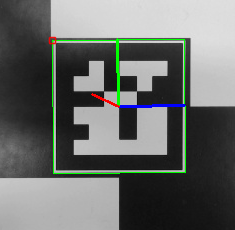
\includegraphics[width=0.4\textwidth]{pictures/aruco_detection.png}
                \caption{Image with detected markers and projected axes.}
            \end{figure}
        \end{center}
    
        \item \textbf{Position Corrections:} 
        Based on the \texttt{tvec} values, the necessary corrections were calculated to adjust the drone's position relative to the marker, including lateral (\textit{x}), vertical (\textit{y}), and depth (\textit{z}) movements.
    
        \item \textbf{System Interaction:} 
        The results of ArUco marker detection were primarily used for real-time visualization of the drone's position and orientation. The system was not designed or implemented for precise landing. However, the detection system provides a foundation for potential future developments involving precise drone landing.
    \end{enumerate}
            
        
\section{Communication System}

    \subsection{Specifications and Requirements} 
    The communication system between the drone, the charging station, and the ground computer is designed to ensure efficient, real-time transfer of critical data. The main requirements are:
    
    \begin{itemize} 
        \item \textbf{WiFi-Based Local Network:} Ensures effective communication between devices without the need for Internet access, creating a secure and self-contained system. 
        \item \textbf{ROS 2 DDS Middleware:} Utilizes ROS 2's distributed node and topic architecture to facilitate robust and reliable data exchange between all connected devices. 
    \end{itemize}
    
    \subsection{Communication Architecture} 
    The system is built on ROS 2's capabilities to enable seamless interaction between devices through nodes and topics. Each component has specific roles and responsibilities within the communication architecture:
    
    \begin{itemize} 
        \item \textbf{Drone:} Acts as a mobile node that: 
        \begin{itemize} 
            \item Publishes compressed camera images (\texttt{/camera\_image/compressed}) for visual processing.
            \item Transmits status data, including battery level, position, and other critical parameters, for real-time monitoring.
        \end{itemize}

        \item \textbf{Ground Computer:} Functions as the control and monitoring hub, running an interface that: 
        \begin{itemize} 
            \item Subscribes to topics published by the drone for processing camera images and calculating the position of ArUco markers. 
            \item Displays drone status information, such as battery level and flight mode, in real-time. 
            \item Publishes control commands to the charging station (e.g., opening or closing the drawer) via dedicated topics. 
        \end{itemize} 
        \item \textbf{Charging Station:} Operates as a stationary node that: 
        \begin{itemize} 
            \item Subscribes to control commands from the ground computer's interface. 
            \item Executes specific actions, such as opening and closing the drawer, to accommodate the drone. 
        \end{itemize} 
    \end{itemize}
    
    \subsection{Key Features} The communication system leverages ROS 2's distributed architecture to provide the following capabilities: 
    \begin{itemize} 
        \item \textbf{Real-time Monitoring:} Enables continuous tracking of drone parameters, ensuring precise and efficient operations. 
        \item \textbf{Concurrent Task Execution:} Supports multithreading to allow simultaneous data processing, camera control, and station operations without delays. 
        \item \textbf{Scalability and Reliability:} Facilitates synchronized operations across multiple devices, ensuring robust communication and rapid response to commands. 
    \end{itemize}
    
    \begin{figure}[H] 
        \centering 
        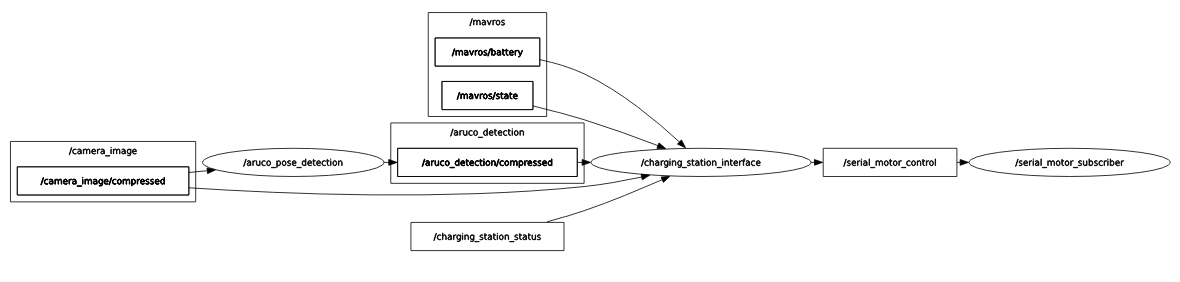
\includegraphics[width=0.8\textwidth]{pictures/complete_node_diagram.png} 
        \caption{Communication diagram showcasing the interaction between devices using ROS 2.} 
        \label{fig:communication_architecture} 
    \end{figure}

    




